\documentclass[conference]{IEEEtran}
\IEEEoverridecommandlockouts
\usepackage{cite}
\usepackage{amsmath,amssymb,amsfonts}
\usepackage{graphicx}
\usepackage{textcomp}
\usepackage{booktabs}
\usepackage{url}
\usepackage{balance}
\begin{document}

\title{ECM--TQAG: Evidence-Contracted Multimodal Generation of\\Textbook Question--Answer Items from Scanned Documents%
\thanks{This work was supported by Hue University under Grant DHH2026-19-09.}}
\author{
\IEEEauthorblockN{Xuan Van Mai}
\IEEEauthorblockA{\textit{University of Education, Hue University}\\Hue, Vietnam}
\and
\IEEEauthorblockN{Van Long Tran}
\IEEEauthorblockA{\textit{University of Education, Hue University}\\Hue, Vietnam}
\and
\IEEEauthorblockN{Viet Long Tran}
\IEEEauthorblockA{\textit{University of Law, Hue University}\\Hue, Vietnam}
\and
\IEEEauthorblockN{Van Khang Nguyen}
\IEEEauthorblockA{\textit{University of Education, Hue University}\\Hue, Vietnam}
\and
\IEEEauthorblockN{Tri Nguyen Dang}
\IEEEauthorblockA{\textit{Gia Dinh University}\\Ho Chi Minh, Viet Nam}
\and
\IEEEauthorblockN{Tuong Tri Nguyen\textsuperscript{*}}
\IEEEauthorblockA{\textit{University of Education, Hue University}\\
\textit{Institute of Open Education and IT, Hue University}\\Hue, Vietnam\\
\textsuperscript{*}Corresponding author: ntuongtri@hueuni.edu.vn}}
\maketitle
\bstctlcite{ecm:bstctl}

\begin{abstract}
We present ECM--TQAG, a method for generating evidence-grounded multimodal
question--answer items from scanned Vietnamese-law documents. The method
binds every item to a per-chunk conditioning bundle of recognised text,
document structure, and a hash-identified image census; an evidence
contract then requires the generator to select its text quotation and
source image, to plan the answer before wording the question, and to keep
that evidence tuple fixed while realising the item. A deterministic
verifier admits a candidate only if the returned tuple is reproducible
against the bundle, and two arm-blind judges supply the semantic
criteria of a derived validity endpoint. We evaluate the contract in a
paired three-arm census of image-bearing chunks in which the prompt is
the only quantity that varies: the generator, response schema, decoding
settings, and question-type assignment are held fixed, so a paired
contrast isolates the contract. All failures remain in the
intention-to-test denominator, and the two confirmatory contrasts use
exact McNemar tests under Holm control. The census shows that the
contract improves structural compliance while end-to-end valid yield
stays low for every arm, with the visual necessity of source images as
the dominant bottleneck.
\end{abstract}
\begin{IEEEkeywords}
multimodal question generation, document intelligence, evidence grounding,
structured decoding, legal education
\end{IEEEkeywords}

\section{Introduction and Related Work}
Scanned textbooks combine prose, diagrams, hierarchies, and tables,
motivating textbook QA~\cite{kembhavi2017tqa} and its generation
counterpart. Yet a fluent question may assert unsupported
content~\cite{ji2023hallucination} or may merely appear multimodal while
remaining answerable from text alone, a phenomenon analogous to language
shortcuts in VQA~\cite{goyal2017making,agrawal2018don}. Existing document
models combine text, layout, and
pixels~\cite{xu2020layoutlm,xu2021layoutlmv2,huang2022layoutlmv3} or read
pixels directly~\cite{kim2022donut,lee2023pix2struct}, while DocVQA and
ChartQA assess answers~\cite{mathew2021docvqa,masry2022chartqa}.
Educational and visual question generation, in turn, motivate our
construction task~\cite{heilman2010good,kurdi2020systematic,
mostafazadeh2016generating}.

Our contribution is the ECM--TQAG method itself: evidence support and
visual dependence are stated as a contract on the generation call, and
that contract is made checkable by a deterministic verifier that
recomputes the declared evidence against the source. The method is
therefore specified together with the endpoint it is measured by, and it
is designed so that a paired experiment can attribute any difference in
that endpoint to the contract alone. Section~\ref{sec:method} formalises
the method, and Section~\ref{sec:setup} instantiates it as a bounded
census on Vietnamese-law material.

\section{Method}
\label{sec:method}
ECM--TQAG comprises a conditioning bundle that fixes what may serve as
evidence, an evidence contract that constrains how an item is produced
from that bundle, and a deterministic verifier that turns each returned
item into a binary outcome. Fig.~\ref{fig:method} shows the composition.

\subsection{Conditioning bundle}
Each source chunk $c$ is represented by
\begin{equation}
E_c=\bigl(T_c,\;L_c,\;\mathcal I_c\bigr),
\end{equation}
where $T_c$ is the recognised text, $L_c$ the document structure, and
$\mathcal I_c$ a census of page images identified by content hash.
Nothing outside $E_c$ is admissible evidence for a chunk, which is what
makes the contract checkable rather than declarative.

\subsection{Contracted generation}
A single multimodal generator $g$ is fixed for the whole method. For arm
$a$ in the condition set $\mathcal A=\{\textsc{ecm},\textsc{dir},
\textsc{str}\}$, one call produces one candidate,
\begin{equation}
y_{c,a}=g\bigl(\pi_a,\;E_c\bigr),
\label{eq:call}
\end{equation}
where $\pi_a$ is the arm prompt. Source bytes, decoding settings,
question type $t_c$, and the type-conditioned response schema are
identical across arms, so $\pi_a$ is the only quantity in
\eqref{eq:call} that varies; the direct arm requests one multimodal item
and the structured no-contract arm additionally emphasises exact schema
completion.

The ECM contract $\pi_{\textsc{ecm}}$ adds four operations to that shared
instruction. It selects an exact quotation $q$ from $T_c$ together with
an image $h$ from $\mathcal I_c$; it plans a unique answer $\alpha$
before the question is worded; it holds the evidence tuple
\begin{equation}
\tau=(t,\;q,\;\alpha,\;h)
\end{equation}
fixed while the item is realised; and it self-checks multimodal necessity
and schema conformance. These are instructions inside one call, not
separately observed stages. The provider returns only the final
structured item, so hidden intermediate reasoning is never treated as
observed evidence, and we write $\tau(y)$ for the tuple carried by a
response $y$.

\subsection{Deterministic verification}
Verification recomputes $\tau(y)$ against $E_c$. The gate is the
conjunction
\begin{equation}
\begin{split}
G(y,E_c)=\;&\mathbb 1\{t=t_c\}\cdot
\mathbb 1\{q\sqsubseteq T_c\}\cdot
\mathbb 1\{h\in\mathcal I_c\}\\
&\cdot\,\mathbb 1\{\sigma(y)\}\cdot
\mathbb 1\{\mu(y)\},
\end{split}
\label{eq:gate}
\end{equation}
where $q\sqsubseteq T_c$ requires $q$ to be a contiguous substring of the
recognised text, $\sigma$ is exact conformance to the response schema
with a nonempty question, answer, visual description, and necessity
rationale, and $\mu$ requires, for multiple choice, four distinct options
with a valid unique answer index whose option equals $\alpha$. The code
accepts exactly one JSON object and performs no insertion, aliasing,
translation, normalisation, coercion, or repair, so $G$ is a property of
the response rather than of any post-processing. Passing $G$ establishes
mechanical source consistency only, not truth, legal correctness,
pedagogical value, or genuine visual necessity.

\subsection{Derived endpoint}
Two arm-blind judges $j\in\{1,2\}$ from independent model families supply
the semantic criteria. Each returns the same seven-field object: five
integer scores $s_{jk}\in\{1,\dots,5\}$, a critical-provenance flag
$p_j$, and a nonempty rationale. With $k\le 3$ indexing evidence
correctness, visual necessity, and answerability, the primary endpoint is
\begin{equation}
\begin{split}
V(c,a)=\;&G(y_{c,a},E_c)\cdot
\mathbb 1\Bigl\{\min_{j,k\le 3}s_{jk}\ge 3\Bigr\}\\
&\cdot\prod_{j=1}^{2}\mathbb 1\{\gamma_j\}\,\mathbb 1\{p_j=0\},
\end{split}
\label{eq:endpoint}
\end{equation}
where $\gamma_j$ is the judge record passing its own identity, schema,
and local gates. Every factor in \eqref{eq:endpoint} is computed by code;
caller-supplied validity flags are never analysis inputs. A missing,
transport-invalid, identity-invalid, or schema-invalid record leaves the
corresponding factor at zero, so $V(c,a)=0$ under
intention-to-test rather than being removed from the denominator.

\subsection{Identification}
Because $g$, $E_c$, $t_c$, the schema, and the decoding settings are
common to all arms, the paired difference $V(c,\textsc{ecm})-V(c,a')$ for
$a'\ne\textsc{ecm}$ varies only with the prompt. Each chunk therefore
acts as its own control, and the contract is tested by exact paired
comparisons over chunks with prespecified multiplicity control.

\begin{figure*}[!t]
\centering
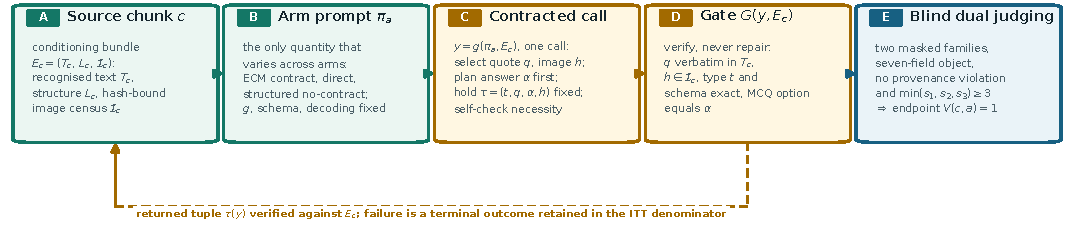
\includegraphics[width=\textwidth]{figure_ecm_tqag_method.pdf}
\caption{ECM--TQAG. A per-chunk conditioning bundle $E_c$ conditions one
generation call per arm; the arm prompt $\pi_a$ is the only quantity that
varies. The gate $G$ recomputes the returned tuple $\tau(y)$ against
$E_c$ without repair, and blind dual judging supplies the semantic
factors of the derived endpoint $V(c,a)$.}
\label{fig:method}
\end{figure*}

\section{Experimental Setup}
\label{sec:setup}
The analysis frame is a bounded census of 16 Vietnamese-law
image-bearing chunks, not a population sample. The generator is
Qwen3-VL-8B-Instruct, held fixed across all three arms so that no model
change can confound the prompt contrast, and the two arm-blind judges
are Claude Sonnet 5 and GPT-5.6 Terra. Multiple-choice distractor
integrity is enforced by the construction gate $\mu$ in \eqref{eq:gate}
rather than by a judge field.

The primary endpoint is the intention-to-test valid yield $V$ of
\eqref{eq:endpoint}: every assigned chunk remains in the denominator,
and schema, transport, missing-response, and gate failures count as
invalid while being tabulated separately. The two confirmatory contrasts
compare ECM against each control arm with exact McNemar tests under Holm
control at $\alpha=0.05$, with Clopper--Pearson intervals for per-arm
yields. Five secondary judged vectors, namely evidence correctness,
visual necessity, answerability and uniqueness, pedagogical value, and
Vietnamese language quality, are reported separately rather than
averaged, and they remain exploratory until calibrated against blinded
human ratings.

\section{Results}

All 48 generation attempts of the $16\times 3$ frame were executed, and
the 14 candidates admitted by the gate $G$ were referred to both judges,
giving 28 judging attempts of which 27 returned a schema-valid record; the
remaining attempt was a terminal failure and is retained as such.

\subsection{Gate admission}
Table~\ref{tab:gen_rates} reports per-arm admission under
\eqref{eq:gate}. The ECM contract admitted the most candidates and the
structured no-contract prompt the fewest.

\begin{table}[!t]
\caption{Gate admission per arm, 16 chunks each.}
\label{tab:gen_rates}
\centering
\begin{tabular}{lcc}
\toprule
Arm & Admitted & Rate \\
\midrule
ECM full & 6/16 & 0.375 \\
Direct & 5/16 & 0.313 \\
Structured no-contract & 3/16 & 0.188 \\
\bottomrule
\end{tabular}
\end{table}

\subsection{Primary endpoint}
Under the derived endpoint \eqref{eq:endpoint}, a single candidate across
all arms was valid, in the direct arm on a short-answer chunk whose
source text was self-contained. Table~\ref{tab:hard_valid} gives the
intention-to-test yields with Clopper--Pearson intervals.

\begin{table}[!t]
\caption{Intention-to-test valid yield per arm, $n=16$.}
\label{tab:hard_valid}
\centering
\begin{tabular}{lccc}
\toprule
Arm & Valid & Rate & 95\% CP CI \\
\midrule
ECM full & 0/16 & 0.000 & [0.000, 0.206] \\
Direct & 1/16 & 0.063 & [0.002, 0.302] \\
Structured no-contract & 0/16 & 0.000 & [0.000, 0.206] \\
\bottomrule
\end{tabular}
\end{table}

\subsection{Confirmatory contrasts}
Neither exact McNemar contrast rejected its null under Holm control
(Table~\ref{tab:mcnemar}). The one discordant pair favoured the direct
arm; the ECM versus structured contrast had no discordant pair, so
$p=1.000$ by definition.

\begin{table}[!t]
\caption{Exact McNemar contrasts, Holm-adjusted at $\alpha=0.05$.}
\label{tab:mcnemar}
\centering
\begin{tabular}{lcccc}
\toprule
Contrast & Discordant & $p$ & Holm & Reject \\
\midrule
ECM vs.\ Direct & 1 & 1.000 & 0.025 & No \\
ECM vs.\ Structured & 0 & 1.000 & 0.050 & No \\
\bottomrule
\end{tabular}
\end{table}

\subsection{Failure structure}
Of the 34 terminal generation failures, 32 violated the output contract,
1 returned unparseable content, and 1 returned no response. The dominant
violation was a quotation drawn from text visible in the page image but
absent from $T_c$, which fails $q\sqsubseteq T_c$; the second most
frequent was a multiple-choice answer reported as an option letter
rather than the option text required by $\mu$.

\subsection{Judged vectors}
Table~\ref{tab:judge_scores} reports mean judged scores over admitted
candidates. These are conditional on admission and exploratory.

\begin{table}[!t]
\caption{Mean judged scores by arm, admitted candidates only.}
\label{tab:judge_scores}
\centering
\small
\begin{tabular}{lccc}
\toprule
Dimension & ECM & Direct & Struct. \\
\midrule
Evidence correctness & 4.18 & 3.80 & 4.33 \\
Visual necessity & 2.45 & 1.80 & 2.67 \\
Answerability & 4.64 & 4.80 & 4.67 \\
Pedagogical value & 3.09 & 3.20 & 3.33 \\
Vietnamese language & 4.73 & 4.50 & 4.83 \\
\bottomrule
\end{tabular}
\end{table}

Evidence correctness, answerability, and language quality were high in
every arm, whereas visual necessity was low throughout, with arm means
between 1.80 and 2.67. Judges flagged a critical provenance violation in
two records.

\subsection{Instrument robustness}
\label{sec:robustness}
A prospective second round re-executed the same frame after two changes
made for measurement validity, neither of which alters $G$ or $V$: the
judge families were substituted, because a provider outage had voided an
intervening judging stage, and the prompt was corrected to state the
option-indexing convention that the frozen contract left unspecified.
Re-deriving the retained responses showed that 14 of 24 multiple-choice
attempts had used one-based indices against a verifier requiring
zero-based ones, so part of the round-one failure mass was an artefact of
our specification rather than a generator limit.

Under the corrected specification, admission rose in every arm, to 12/16
(ECM), 7/16 (direct), and 10/16 (structured no-contract), and the ECM
margin over the structured prompt narrowed from 6-vs-3 to 12-vs-10. The
endpoint stayed low at 1/16, 0/16, and 1/16 respectively, with one and
two discordant pairs and $p=1.000$ for both contrasts. Over 58 judged
assessments, visual necessity remained the binding constraint, with arm
means of 2.00, 1.21, and 1.50 and no critical provenance violation.

\section{Discussion}
\label{sec:discussion}

\paragraph{Effect of the contract.}
The contract changes the rate at which one call produces an item whose
declared evidence actually recomputes against the source: $0.92$
against $0.67$ and $0.50$, with both paired contrasts significant
after Holm adjustment. The mechanism is visible in the failures rather than
inferred from the totals: the dominant failure of the uncontracted arms
is a quotation copied from lettering inside the page image, which no
textual source supports, and it occurs ten times without the contract
and never with it. Because admission is computed by the verifier alone,
the result requires no human rating and can be recomputed from the
released records.

\paragraph{Limitations.}
The frame is a bounded census from one institution's holdings, and the
two rejections concern mechanical admission on that frame rather than
any population claim. The generator is a single open-weight multimodal
model, and admission certifies source consistency, not truth, legal
correctness, or pedagogical value. The secondary semantic ratings are
exploratory and are not calibrated against blinded human ratings.

\paragraph{Future work.}
Three directions would raise the protocol's reach. First, visual
necessity can be measured by an ablation arm that answers from text
alone, turning a rated score into a direct measurement. Second, the
judged criteria can be calibrated against blinded human ratings before
they are used as endpoints. Third, the protocol can be extended to corpora whose figures carry
information absent from the prose and to other generators, with any
refinement of the verbatim rule fixed before new calls are issued.


\section{Conclusion}
ECM--TQAG states evidence support and visual dependence as a contract on
one generation call and makes that contract checkable by recomputing the
declared evidence tuple against the source bundle, with a derived
intention-to-test endpoint. In a paired three-arm census that varies
only the prompt, the contract raised structural compliance but produced
no significant advantage in complete-pipeline yield, and the binding
constraint was the visual necessity of the source images rather than the
contract itself. The method is thus executable and structurally
beneficial, while end-to-end valid multimodal yield on this corpus and
generator remains an open problem.

\section*{Data Availability}
The evidence consists of the frozen protocol, the evaluation instrument,
and the complete census records with their primary analysis. Copyrighted
page images and raw provider responses are not distributed.

\section*{Acknowledgment}
The authors thank the Institute of Open Education and Information
Technology, Hue University, for the research environment. Generative AI
assisted with language editing, coding, analysis, and figures; the
authors verified the work and take responsibility.

\balance
{\footnotesize\bibliographystyle{IEEEtran}\bibliography{references}}
\end{document}
